\documentclass[../../lecture_notes.tex]{subfiles}
\begin{document}



This is a new field, so the terminology is not well defined — the ideas are what is important. We define \term{cloud computing} as computation done on a network of servers maintained by a cloud service provider

With our model of cloud computing, our goal is effortless elasticity. We can measure this with a few heuristics:
\begin{itemize}
	\item scalability $\coloneqq$ (ability to change size)
	\item availability $\coloneqq$ (ability to run even with failure)
	\item fault tolerance $\coloneqq$ (transparent availability)
	\item configuration $\coloneqq$ (ease of setup)
	\item Quality of Service
	\item QoS Monitoring Quality
\end{itemize}
Note: developers often believe the STATE is not part of the QoS metrics but providers disagree.

Cloud computing can be used to the benefit of IOT/Edge Computing, since many home devices now connect to the internet and cannot do heavy computation.

To speed up our computing we use \term{Fog Computing}.

\begin{figure}[h!]
	\centering
	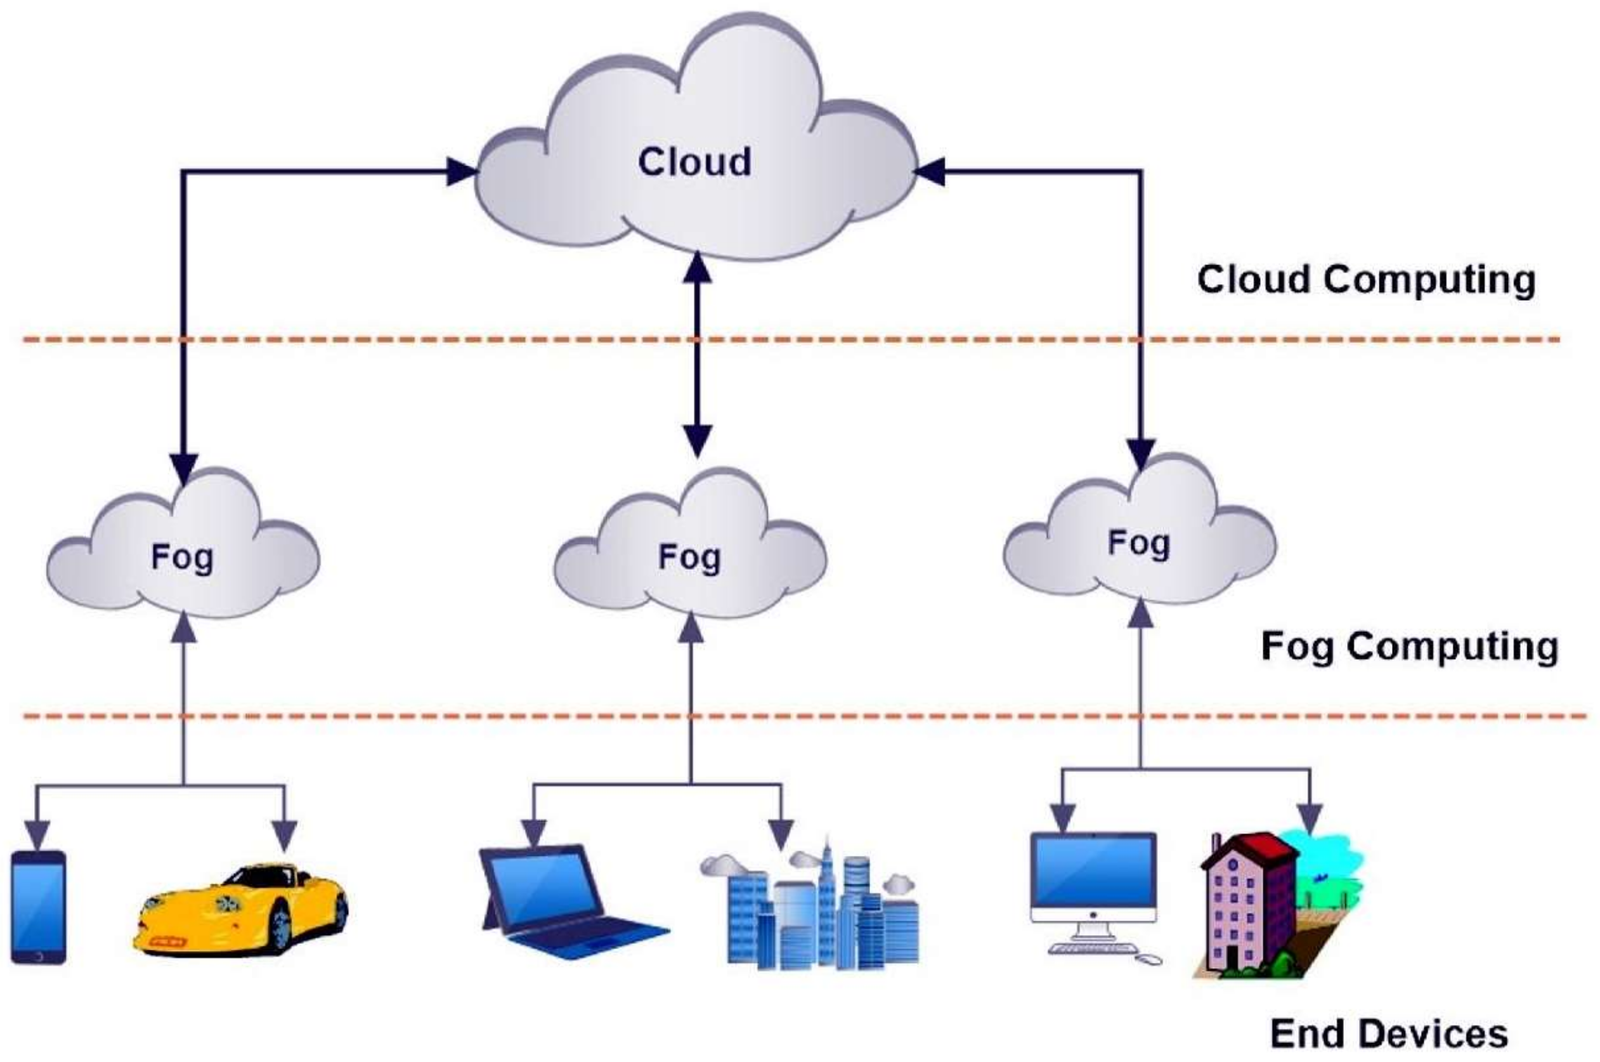
\includegraphics[width=0.75\linewidth]{cloud}
\end{figure}

\begin{itemize}
\item localized nodes provide a hybrid between the device and the cloud
\item the cloud functions like a cache for computation
\item this forms a computation hierarchy
\end{itemize}

We want to make this \term{transparent} $\coloneqq$ to hide the servers from developers entirely, so we run provided functions in the servers, and developers are billed on usage, and it scales to \$0.

\subsection*{Models of Cloud Computing}

\subsubsection*{Function at a Service (FaaS)}
\begin{itemize}
\item A function is the primary unit of computation.
\item Functions are executed in response to a trigger (such as an HTTP/HTTPS request).
\item Rules:
	\begin{itemize}
		\item a function must execute relatively quickly
		\item a function can have no persistent state
		\item functions can, however, refer to storage or database servers to find a state)
	\end{itemize}
\end{itemize}

For an example of FaaS, consider:
\begin{lstlisting}
function main(params, context) {
	return { payload: 'Hello ' + params.name };
}
// params and context are JSON objects: a marshaling of a data structure
// context is a JSON object that represents metadata like security
\end{lstlisting}

If we are worried about performance, we would never use FaaS: (un)marshaling is slow. We instead use FaaS for processing speed or functionality.

\begin{center}
\resizebox{\textwidth}{!}{
\begin{tikzpicture}
\node[rectangle, minimum width=2cm, minimum height=1cm, draw] (UI) {UI};
\node[below=of UI, rectangle, minimum width=2cm, minimum height=1cm, draw, align=center] 
	(EH) {Event\\Handler};
\node[below=of EH, rectangle, minimum width=2cm, minimum height=1cm, draw, align=center] 
	(API) {API\\Gateway};
\node[right=of EH] (MID) {}; 
\node[above=3cm of MID] (U) {edge master};\node[below=3cm of MID] (B) {};\draw (U) -- (B);
\node[right=of MID] (EQ) {\huge\begin{tabular}{| c | c | c | c |}\hline & & & \\\hline\end{tabular}};
\node[right=of EQ, rectangle, minimum width=3cm, draw] (DIS) {Dispatcher};
\node[right=of DIS, rectangle, minimum width=2cm, minimum height=1cm, draw] (W1) {Worker};
\node[below=of W1, rectangle, minimum width=2cm, minimum height=1cm, draw, align=center] 
	(W2) {Worker};
\node[above=of W1, rectangle, minimum width=2cm, minimum height=1cm, draw, align=center] 
	(W3) {Worker};
\node[right=of W1, star, star points=10, minimum size=1cm, draw] {STATE};
\draw[Latex-] (API.west) -- node[above] {\scriptsize Environment} +(-2,0);
\draw[-Latex] (UI) -- (MID); \draw[-Latex] (EH) -- (MID); \draw[-Latex] (API) -- (MID);
\draw[-Latex] (MID) -- (EQ); \draw[-Latex] (EQ) -- (DIS); 
\draw[-Latex] (DIS) -- (W1); \draw[-Latex] (DIS) -- (W2); \draw[-Latex] (DIS) -- (W3);
\end{tikzpicture}
}
\end{center}


The steps of event execution are:
\begin{enumerate}[nosep]
\item arrival
\item validation
	\begin{enumerate}[nosep]
		\item authentication
		\item authorization
		\item resource limit checking
	\end{enumerate}
\item enqueue
\item dispatch
\item allocate a container (a cheap VM)
\item copy function code into the container *
\item execute the function
\item deallocate the container
\end{enumerate}
* our bottleneck is here, since Linux booting is slow relative to all the other operations.

This is called the \term{cold start problem}.
	\begin{itemize}
		\item This causes our latency to skyrocket.
		\item We can temper the throughput by adding more workers, but how do we temper latency?
			\begin{itemize}
				\item pre-load stem cell containers with modules we expect to use
				\item do not clear warm containers post use
			\end{itemize}
		\item We can get to an almost reasonable speed with these techniques!
	\end{itemize}
	
We call this model the \term{Action and Trigger Model}
\begin{itemize}
	\item An event triggers the execution of an action.
	\item One event can trigger multiple actions. We can use this to implement parallel execution.
	\item One action can triggers an action. We can use this to implement serialized execution
	\item this has problems:
		\begin{itemize}
			\item debugging
				\begin{itemize}
					\item GDB is too big to use! We have to use their logs!
				\end{itemize}
			\item fixing bottlenecks
				\begin{itemize}
					\item We can’t use ps! We have to check usage in the logs post-run!
				\end{itemize}
			\item atomicity(?)
				\begin{itemize}
					\item We are sometimes guaranteed atomicity of function calls
				\end{itemize}
			\item change
				\begin{itemize}
					\item We have difficulty refactoring (breaking functions) and reverting to old versions.
					\item The tools are evolving too quickly for us to get used to them!
				\end{itemize}
		\end{itemize}
\end{itemize}


We have a few other basic models of cloud computing which provide different levels of services


\subsubsection*{Infrastructure as a Service (IaaS)}
\begin{itemize}
	\item The provider provides supples virtual machines
	\item A stripped OS called a hypervisor hosts each VM; common ones include Zen and Virtual Box
	\item The programmer is responsible for the OS, configuration, and applications
	\item This is 2/3 of enterprise level IT spending. Security concerns keep it from reaching \%100.
	\item There are some major issues, though:
	\begin{itemize}
		\item We have to anticipate resource usage.
		\item It is hard to adjust usage on the fly.
	\end{itemize}
\end{itemize}


\subsubsection*{Platform as a Service (PaaS)}
\begin{itemize}
	\item The provider supplies some of the software stack in addition to VMs
	\item Less expertise is needed, but provisioning is still pushed on the developer
	\item Developers still have to autoscale.
\end{itemize}


\subsubsection*{Backend as a Service (BaaS)}
\begin{itemize}
	\item the provider supplies a framework for an (often mobile) app on the backend and client
	\item avoids heavy computation on mobile devices
	\item scales, but allows little flexibility
\end{itemize}


\subsubsection*{Software as a Service (SaaS)}
\begin{itemize}
	\item provider supplies the entire platform and stack
	\item the developer calls the service’s API (which is application specific)
	\item can be tailored with callbacks in config files
\end{itemize}

\begin{center}
\begin{tikzpicture}[scale=2]
\begin{axis} [ axis lines=none, ticks=none, axis equal image ]
\addplot[opacity=0, domain=-1:11] {0};
\addplot[domain=0:5] {6/5*x};
\addplot[domain=5:10] {6 - 6/5*(x-5)};
\addplot[domain=0:10, name path=bot] {0};
\addplot[domain=5/3:25/3, name path=mid] {2};
\addplot[domain=10/3:20/3, name path=top] {4};
\addplot[fill=gray] fill between[of=bot and mid];
\addplot[fill=white!50!gray] fill between[of=mid and top];
\node at (5, 1) {\huge IaaS}; \node at (5, 3) {\huge PaaS}; \node at (5, 4.75) {\huge SaaS};
\node[rounded rectangle, fill=white] at (1.5, 1) {Server Storage Network};
\node[rounded rectangle, fill=white, align=center] at (1.5, 15/5) {OS \& Application Stack\\Server Storage Network};
\node[rounded rectangle, fill=white, align=center] at (1.5, 24/5) {Packaged Software\\OS \& Application Stack\\Server Storage Network};
\node[rounded rectangle, fill=white, align=center] at (8.5, 1) {Infrastructure \&\\Network Architects};
\node[rounded rectangle, fill=white, align=center] at (8.5, 15/5) {App Developers};
\node[rounded rectangle, fill=white, align=center] at (8.5, 24/5) {End Users};
\end{axis}
\end{tikzpicture}
\end{center}

Our models form a pyramid of increasing ease but decreasing flexibility.


\end{document}